%% ****** Start of file aiptemplate.tex ****** %
%%
%%   This file is part of the files in the distribution of AIP substyles for REVTeX4.
%%   Version 4.1 of 9 October 2009.
%%
%
% This is a template for producing documents for use with 
% the REVTEX 4.1 document class and the AIP substyles.
% 
% Copy this file to another name and then work on that file.
% That way, you always have this original template file to use.

%\documentclass[aip,jap,numerical,preprint]{revtex4-1}
\documentclass[twocolumn,secnumarabic,amssymb, nobibnotes, aps, pra]{revtex4}
\newcommand{\revtex}{REV\TeX\ }
\newcommand{\classoption}[1]{\texttt{#1}}
\newcommand{\macro}[1]{\texttt{\textbackslash#1}}
\newcommand{\m}[1]{\macro{#1}}
\newcommand{\env}[1]{\texttt{#1}}
\setlength{\textheight}{9.5in}

\usepackage{amsmath}
\usepackage{graphicx}
\usepackage{booktabs}
\usepackage{color}
\usepackage{enumerate}
\providecommand{\e}[1]{\ensuremath{\times 10^{#1}}}

%\draft % marks overfull lines with a black rule on the right

\begin{document}

%Title of paper
\title{$e/m$
% \large{Methods of experimental physics} \\ 
 %\normalsize{PHYS 413}
 }

% repeat the \author .. \affiliation  etc. as needed
% \email, \thanks, \homepage, \altaffiliation all apply to the current
% author. Explanatory text should go in the []'s, actual e-mail
% address or url should go in the {}'s for \email and \homepage.
% Please use the appropriate macro foreach each type of information

% \affiliation command applies to all authors since the last
% \affiliation command. The \affiliation command should follow the
% other information
% \affiliation can be followed by \email, \homepage, \thanks as well.
\author{Jason Morgan}
%\email[]{Your e-mail address}
%\homepage[]{Your web page}
%\thanks{}
%\altaffiliation{}
\affiliation{Department of Physics, Old Dominion University, Norfolk VA 23529}

%\author{H. Hagood}
%\affiliation{Department of Physics, Old Dominion University, Norfolk VA 23529}


\date{April 29, 2014}


\begin{abstract}
This experiment measures the charge to mass ratio of the electron.  The mass ratio is determine by measuring the radius of the circle made by a beam of electrons ecposed to an electric and magnetic field.
\end{abstract}

\maketitle
\section{Introduction}

A magnetic field $\vec{B}$ produced a force $\vec{F}$ on a particle of charge e moving at velocity $\vec{v}$ that is given by the following equation:

\begin{equation}
\vec{F} = e\vec{v} \times \vec{B}
\label{eq:one}  
\end{equation}

This force caused the particle to follow a spiral path since the direction is always perpendicular to the velocity.  The radius of the circle r can be determined by the equilibrium of the magnetic and centripetal forces:

\begin{equation}
evB = \frac{mv^2}{r}
\label{eq:two}  
\end{equation}

\begin{equation}
r = \frac{mv}{eB}
\label{eq:three}  
\end{equation}

m is the mass of the particle.  The last equation we need to arrive and expression for $\frac{e}{m}$ is the kenetic energy a charged particle aquires when falling through a potential difference V:

\begin{equation}
eV = \frac{1}{2}mv^2
\label{eq:four}  
\end{equation}

Solving this for $v^2$ and substituting into equation \ref{eq:three} we arrive at

\begin{equation}
\frac{e}{m} = \frac{2V}{B^2r^2}
\label{eq:em}  
\end{equation}


\section{Experimental setup and procedures}

\begin{figure}[t]
\begin{center}
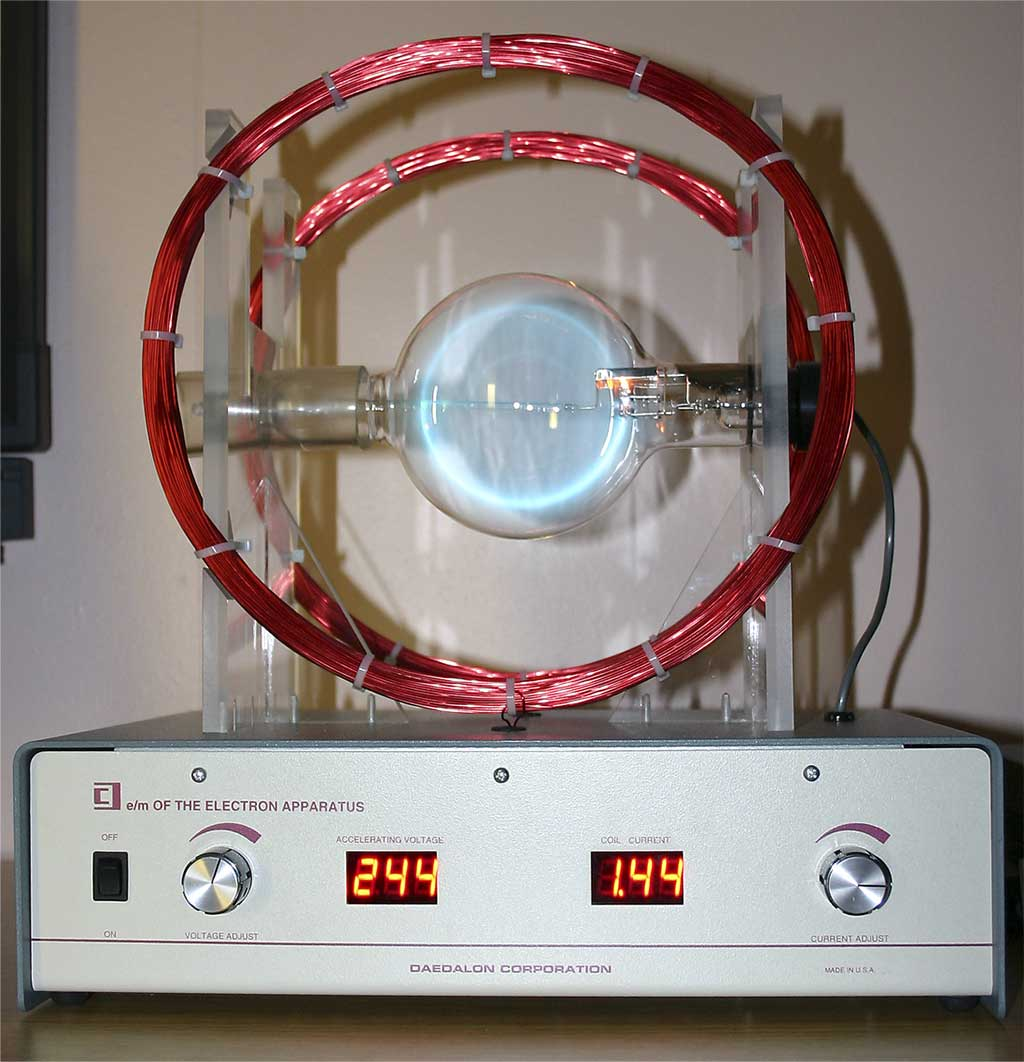
\includegraphics[scale=.2]{e_over_m.jpg}
\end{center}
\caption{$\frac{e}{m}$ appatatus used in this experiment}
\label{fig:setup}
\end{figure}


Equation \ref{eq:em} contains three independent variables.  Three dataset sets were collected where one parameter was held constant and the other two were varied.  The resulting data was then plotted sothat the slope of the line could be used to find the value of $\frac{e}{m}$.  

For the first trial, the accelerating voltage was held at 146.6 $\pm$ 0.1 V. The current to the helmholtz coil were then varied and the resulting current and radius were recorded (Fig. \ref{fig:one}).  The second data set held the helmholtz coil current at 1.6 $\pm$ 0.1 A and the and the accelerating voltage was varied.  The results voltage and radius were recorded (Fig. \ref{fig:two}).  The was repeated a third time holding the radius constant at 0.06 $\pm$ 0.005 m.  The coil current and accelerating voltage were varied and recorded (Fig. \ref{fig:three}).  



\section{Results and Discussion}

Converting the slopes found by plotting the data in R to values of $\frac{e}{m}$ results in the values in table \ref{tab:tuning}.

\begin{table} [h]  % Capital letters stronger suggestion
\caption{Results}      %title of the table     
\centering              % centering table
\begin{tabular}{crr} % creating four columns (c stands for ceneter, r for right, l for left)
\hline\hline %inserting double-line
  e/m & \% Difference   \\
\hline % inserts single-line
$1.67 \times 10^11 \pm 2 \times 10^9$ & 5.0   \\
$1.69 \times 10^11 \pm 1 \times 10^9$ & 3.8   \\
$1.69 \times 10^11 \pm 1 \times 10^9$ & 3.8   \\
\hline % inserts single-line
\end{tabular}
\label{tab:tuning}
\end{table}


The data agrees with the accepted value of 1.761011 ($C/kg$) to with in 5.0\%.  The percent differences for all trials are between 3.8\% and 5.0\%.

\section{Conclusion}

This experiement was a great experience is working with electromagnetism to find the electron charge to mass ration.  The data was consistent for each method of calculating $\frac{e}{m}$ and fits the expected values very well.

\begin{figure}[b]
\begin{center}
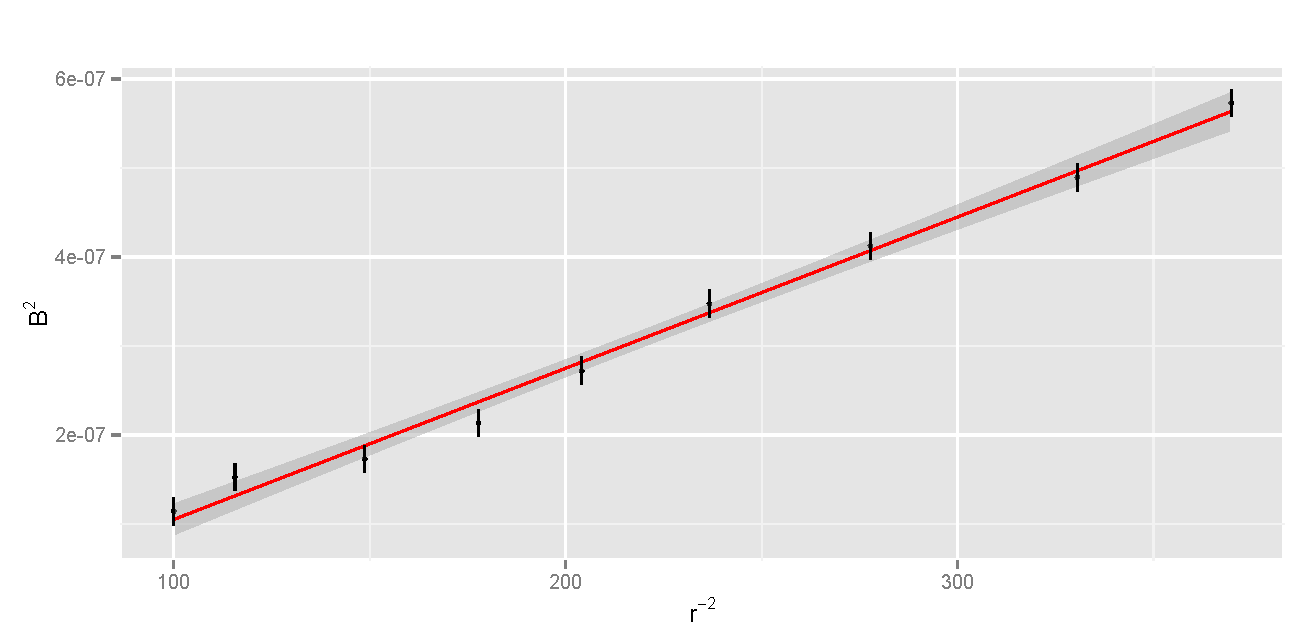
\includegraphics[scale=.8]{plot1.pdf}
\end{center}
\caption{Graph of $B^2$ vs $\frac{1}{r^2}$.  Slope: $1.70\e{-09} \pm 6\e{-11}$ $R^2 = 0.990$. Accelerating voltage held at 146.6 V}
\label{fig:one}
\end{figure}

\begin{figure}[b]
\begin{center}
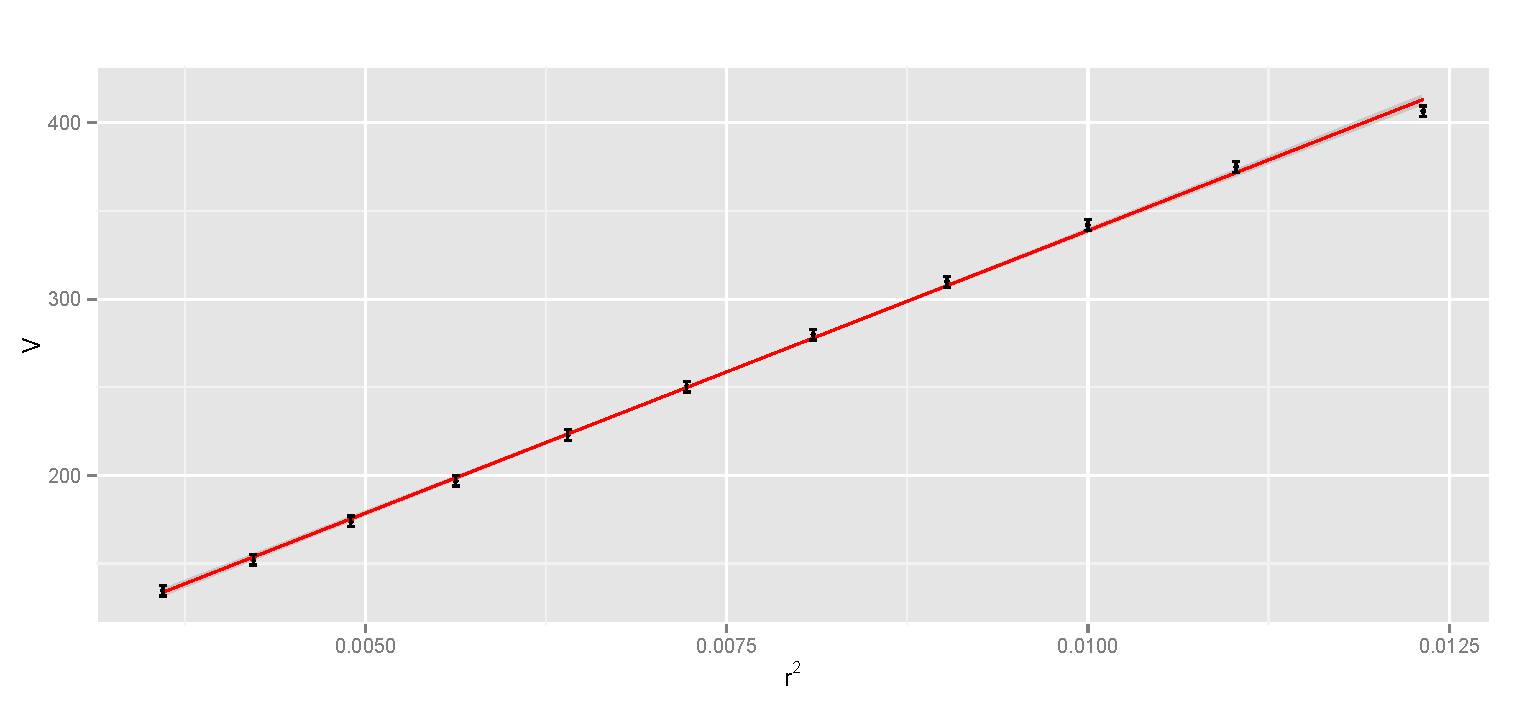
\includegraphics[scale=.7]{plot2.pdf}
\end{center}
\caption{Graph of $V$ vs $r^2$.  Slope: $3.21\e{4} \pm 3\e{2}$ $R^2 = 0.999$.  Coil Current held at 1.60 A}
\label{fig:two}
\end{figure}

\begin{figure}[b]
\begin{center}
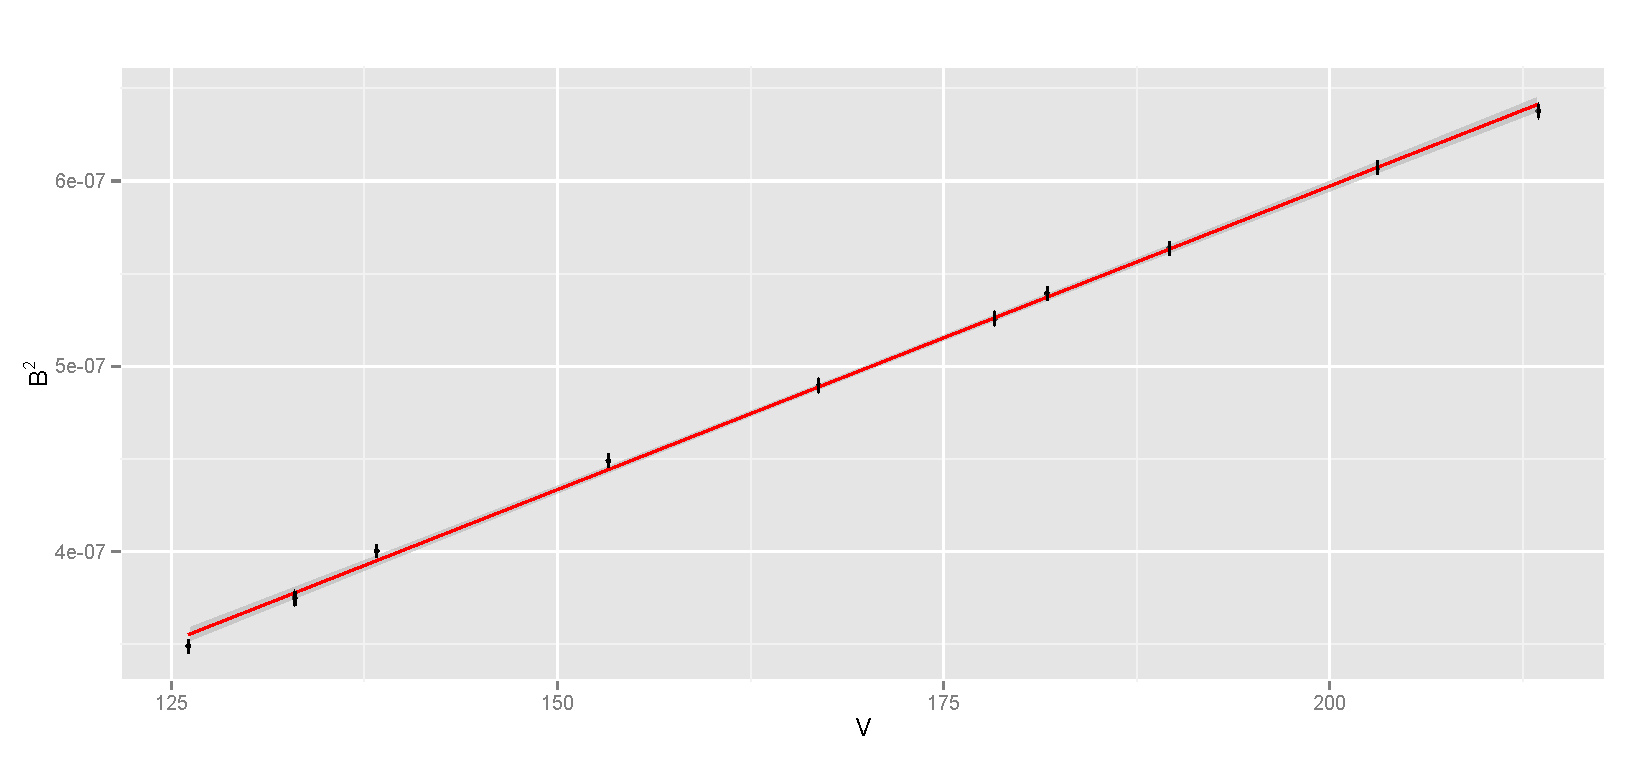
\includegraphics[scale=.6]{plot3.pdf}
\end{center}
\caption{Graph of $B^2$ vs $\frac{1}{r^2}$.  Slope: $3.28\e{-09} \pm 4\e{-11}$ $R^2 = 0.999$. Radius held at 0.06 m}
\label{fig:three}
\end{figure}

%Write down references
%-----------------------------------
\begin{thebibliography}{5}

\end{thebibliography}

\end{document}

%
% ****** End of file aiptemplate.tex ******
